\documentclass[11pt]{article}

\usepackage[margin=1in]{geometry}
\usepackage{outlines}
\usepackage{graphicx}
\usepackage[T1]{fontenc}
\usepackage{subcaption}

\usepackage{geometry}

\usepackage[square,sort,comma,numbers,super]{natbib}

\usepackage{pdflscape}

\usepackage{hyperref}

\usepackage{afterpage}

\graphicspath{ {./images/} }


\setlength{\parindent}{0pt}


% pt = project title; shorthand
\newcommand{\pt}{Multi-User Poker Game}
\newcommand{\pn}{Rekop}

\title{Project Proposal: \pt}
\author{James Scully}

\begin{document}

{\fontfamily{cmss}\selectfont


\hspace{0pt}

\vfill

\begin{center}
	
\includegraphics[scale=0.4]{uni_logo}
	
	\vspace{1cm}
	
	{\Large \textbf{Project Proposal:} \pn \ Poker} \linebreak
	
	\begin{large}
		James Scully (4304469) \\
		psyjs20@nottingham.ac.uk \\
		G400 Computer Science \\
	\end{large}
	
\end{center}

\vfill

\begin{center}
	\textbf{Project Supervisor:} Milena Radenkovic
\end{center}

\hspace{0pt}

\pagebreak

\section*{Background and Motivation}

Poker is a game loved by many around the world twice over and as such has found its way into mobile applications. Many of these do not give control to the players, and are much like in real life, focused on money, rather than a casual and relaxed game. Zynga Poker for example, has been criticized in the past for "throwing too many unwanted features" in the way of the playing the game, despite seeing an increase in revenue. \cite{zynga_unwanted} \\

A quick search of the Google Play Store reveals 250 poker applications, however most of these include some form of monetization whereby the player is likely to purchase chips in order to continue playing, when they have lost all of their chips. Many people prefer mobile games to be simple, easy to use and not plagued with offers for in-game products. They also typically use misleading labels or actions in order to promote these purchases, as seen in Fig 1.


\begin{center}

\begin{figure}[h]
	\makebox[\textwidth][c]{
	\begin{subfigure}[h]{0.6\textwidth}
		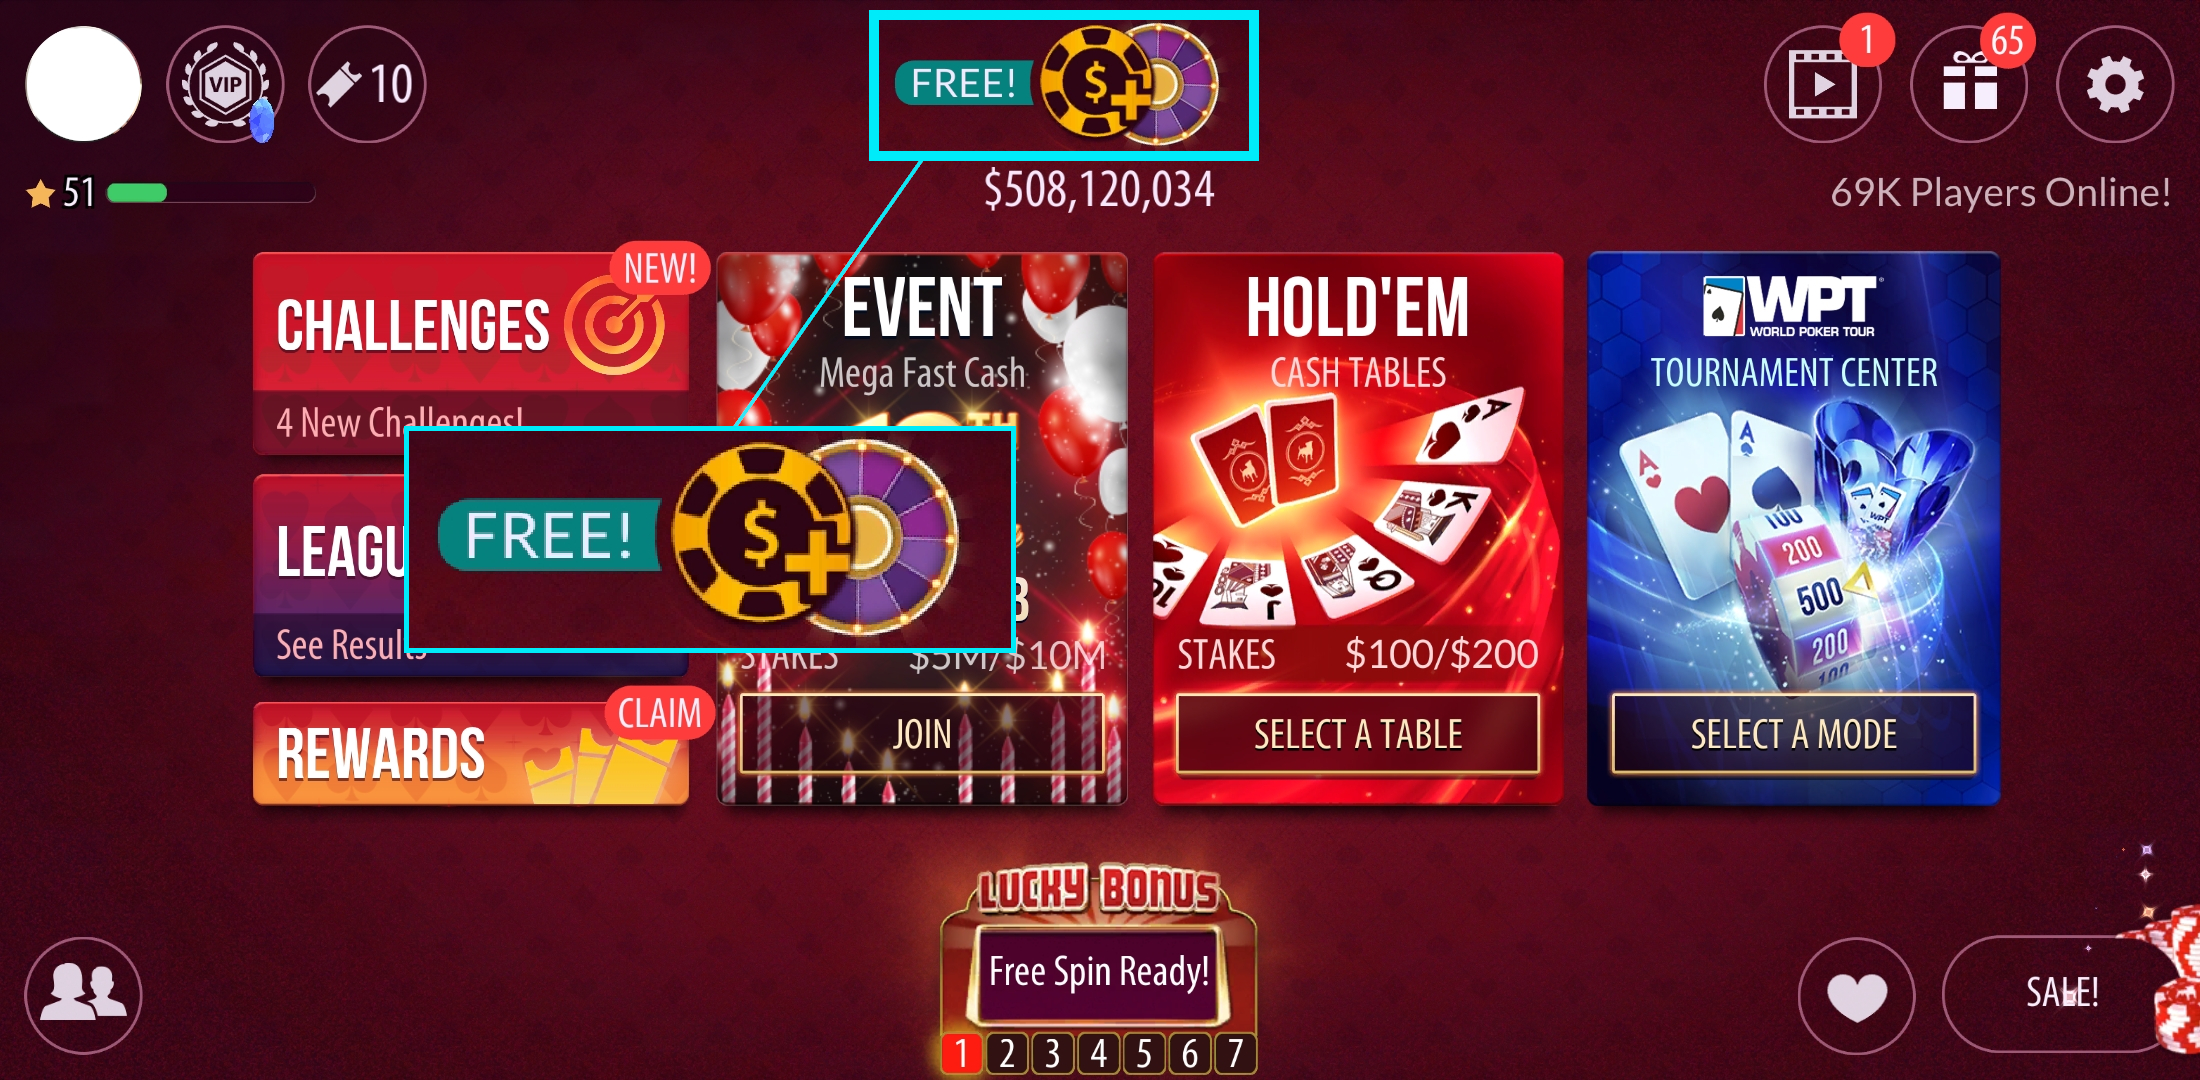
\includegraphics[width=\textwidth]{zynga_before_free_edit}
		\caption{Label insinuating 'FREE' chips}
	\end{subfigure}	
	~
	\begin{subfigure}[h]{0.6\textwidth}
		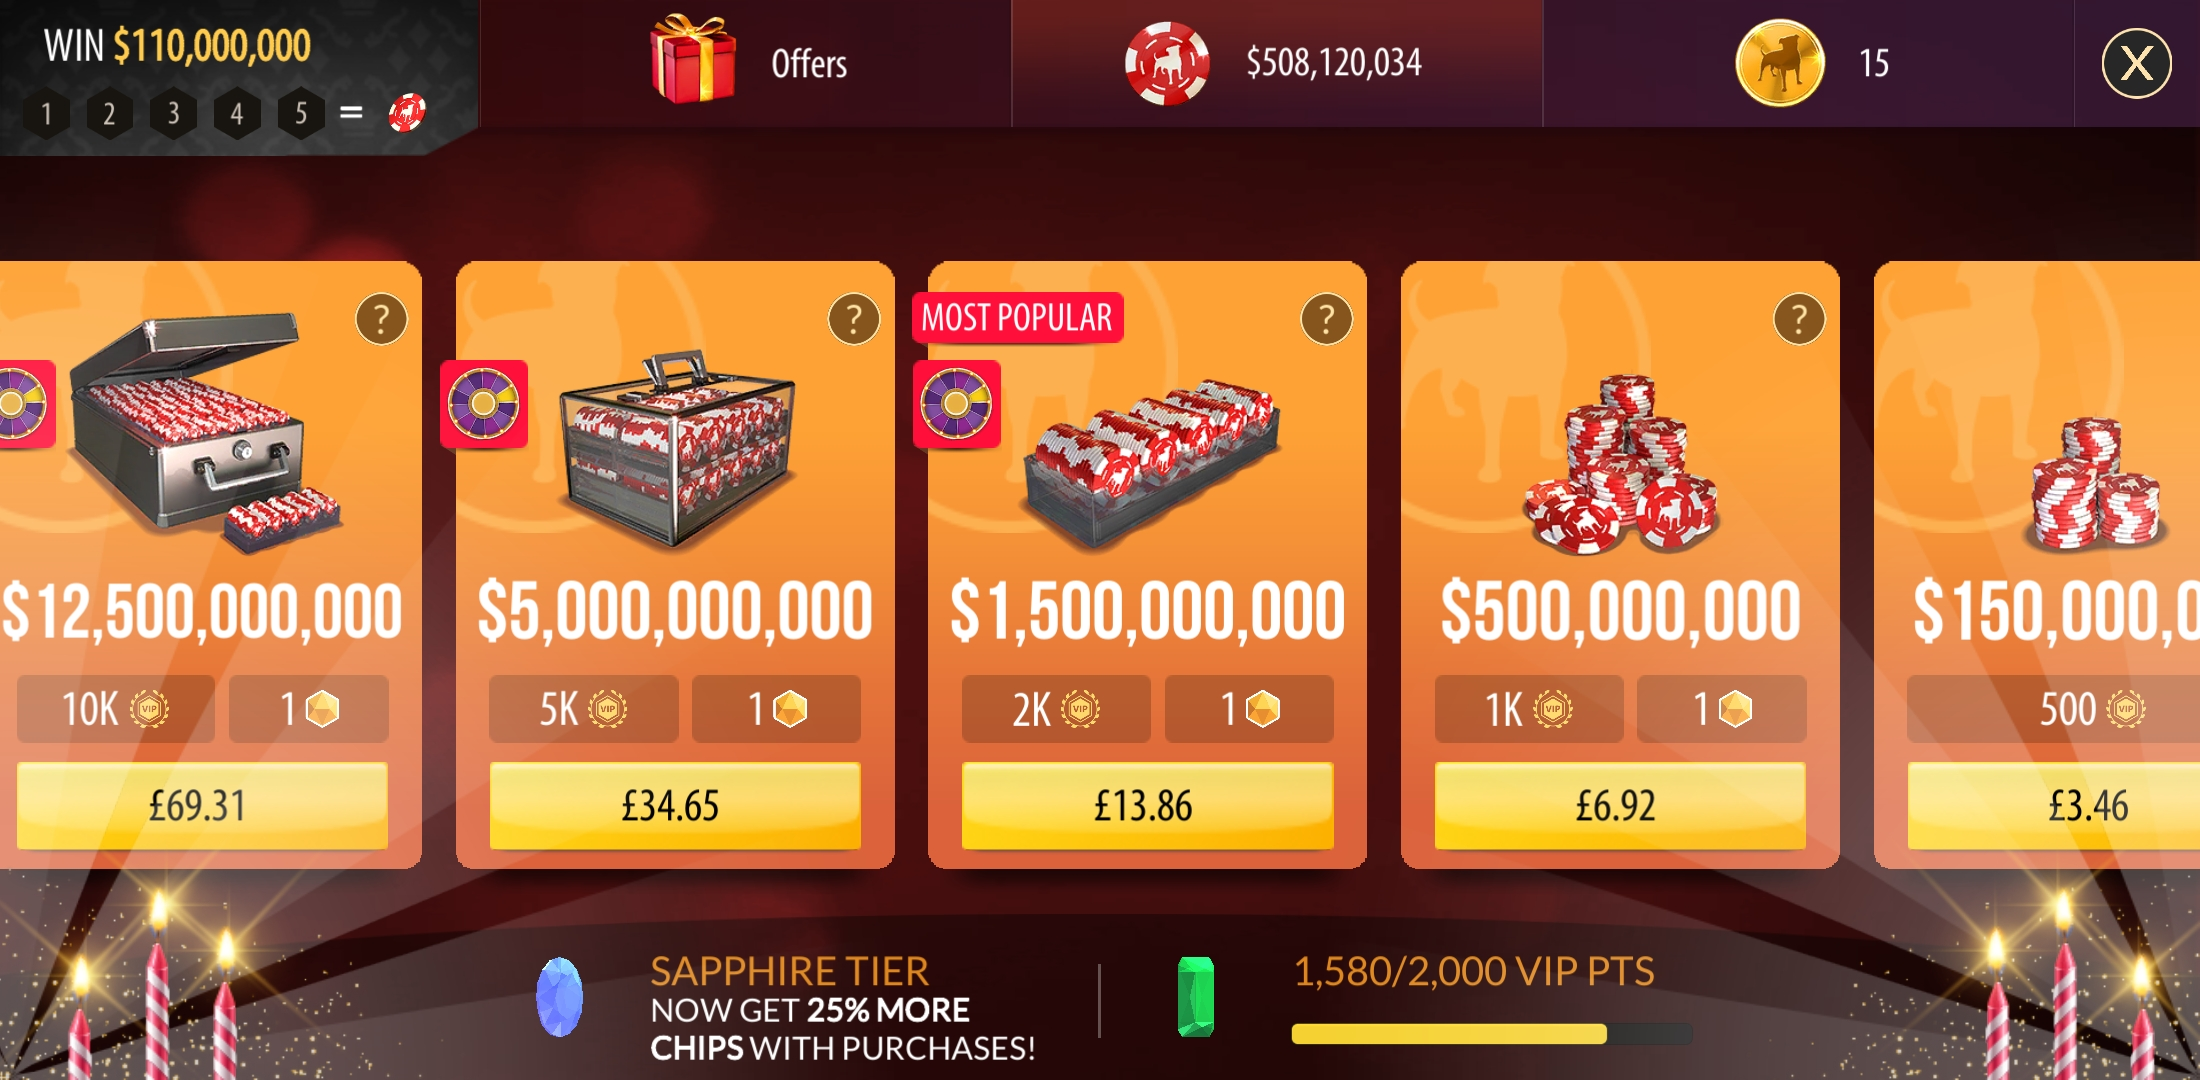
\includegraphics[width=\textwidth]{zynga_after_free}
		\caption{A multitude of purchases}
	\end{subfigure}	
	}
	
	\caption{A common deception used in popular poker applications}
	
\end{figure}
	
\end{center}

As mentioned previously, many of these do not give much control to the user, such as customizing match settings, or the ability to host their own server/lobby to play on. In existing apps, most only have presets and are at the hands of the developers. In regards to user experience, it is best to offer control to the user, as they can tailor the game to their likings. This effect can be seen in a variety of areas not limited to software; think having clothes fit to ones preferences, or the ability to make changes to a home. \cite{customize} % https://www.nngroup.com/articles/customization-personalization/

\newpage
\section*{Aims and Objectives}

The aim of this project is to create a mobile, multi-player poker game as well as a server for people to host their lobbies. 

With this in mind, we have some key objectives to consider: 

\begin{outline}
	\1 Players are able to view multiple statistics:
		\2 Previous hands dealt
		\2 Total win / losses
		\2 Accumulated wins	
	
	\1 Develop a server application which: 
		\2 Handles disconnections / interruptions gracefully
		\2 Is open-source and can be used by the public for private servers
		\2 Is cross-platform, to ensure it is portable.
	\1 Hands that are given out should not be repeated or predictable i.e. near-complete randomness (not time-based seeds)
\end{outline}

\section*{Work plan}


\subsection*{Research and Plan Documents}

Firstly, research will need to be undertaken on areas to innovate upon and frameworks to be used within the app itself, for example if a game engine is going to be used - if so, what API level does it support? How will we host an official server for players to connect to? Next, we'll have to produce requirements; how we're going to meet our key objectives, and ideal features. This will be explained further with the vision and scope document which provides a general vision of a sufficient system and gives an idea of how many features need to be implemented (scope) to prevent feature creep.


\subsection*{Methodology and On-going processes}

This project is going to be developed alongside other studies and as such will be obstructed by other pieces of coursework at some points. Because of this, the Agile methodology will be used as this allows for more flexible deadlines and progress. Other more "rigid" methodologies such as Waterfall are not suitable as game development is a \textbf{\textit{very}} iterative process, not linear. \cite{iterative} \\ 

% https://jserd.springeropen.com/articles/10.1186/s40411-016-0032-7
% https://www.gdcvault.com/play/1013175/Agile-Methodology-in-Game-Development

It is also imperative that a task management system is to be used such as GitHub issues; this will allow for the project to be easily picked up from a certain point and continued, as there will be a few phases where focus on the project will need to be diverted briefly. \\

A journal will be kept on the repository for documenting choices made, problems encountered to aid in developing the interim report and dissertation. \\

\subsection*{Testing and Evaluation}

In similar fashion to the journal, development will include regular unit tests on the back-end and can be integrated into Continuous Integration (CI), as this will generate a pass or fail on the unit tests with each commit. However, this mustn't be compared to a Test-Driven Development (TDD) approach, whereby we would write strictly write tests before actual programming, as we do not have too much time to write tests and develop a fully-functional program; using a TDD approach would not help with meeting deadlines. \cite{tdd_productivity}   \\

% https://www.sciencedirect.com/science/article/pii/S0950584903002040#aep-section-id36

For the front-end, slightly less frequent testing will be done in the form of black/white box testing as automated unit tests are not suitable for user interfaces. 

Evaluation towards the end of development will incorporate feedback from users, findings from quality reviews (both code and user interface). 


\renewcommand\refname{Bibliography}
\begin{thebibliography}{9}

\bibitem{zynga_unwanted}
\begin{flushleft}
	Jeff Grubb,
	\textit{Zynga stock price jumps 7\% as new chief executive replaces Pincus}, 
	1 Mar 2016 \\
	Retrieved from \url{https://venturebeat.com/2016/03/01/zynga-stock-price-jumps-8-as-new-chief-executive-replaces-pincus/}
\end{flushleft}

\bibitem{customize}
\begin{flushleft}
	NNGroup; Amy Schade,
	\textit{Customization vs. Personalization in the User Experience}, 
	10 Jul 2016 \\
	\textit{Why Customize?}	\\
	Retrieved from \url{https://www.nngroup.com/articles/customization-personalization/}
\end{flushleft}

\bibitem{iterative}	

\begin{flushleft}
	Henna-Riikka Ruonala,
	\textit{Agile Game Development: A Systematic Literature Review}, 
	22 Nov 2016, \\
	5.3 Use of Agile Methods; Page 22 \\
	\url{https://pdfs.semanticscholar.org/4bb7/66bee969dd51a5d48ad880523ed475e7c773.pdf}
\end{flushleft}

\bibitem{tdd_productivity}
\begin{flushleft}
	Boby George \& Laurie Williams, 
	\textit{A structured experiment of test-driven development}, 
	15 Apr 2004, \\
	Retrieved from \url{https://www.sciencedirect.com/science/article/pii/S0950584903002040#aep-section-id36}
\end{flushleft}
	
\end{thebibliography}

\newpage

\newgeometry{a4paper,left=0in,right=0in,top=0in,bottom=0in,nohead}


\begin{landscape}
	\begin{center}
		\makebox[\textwidth][c]{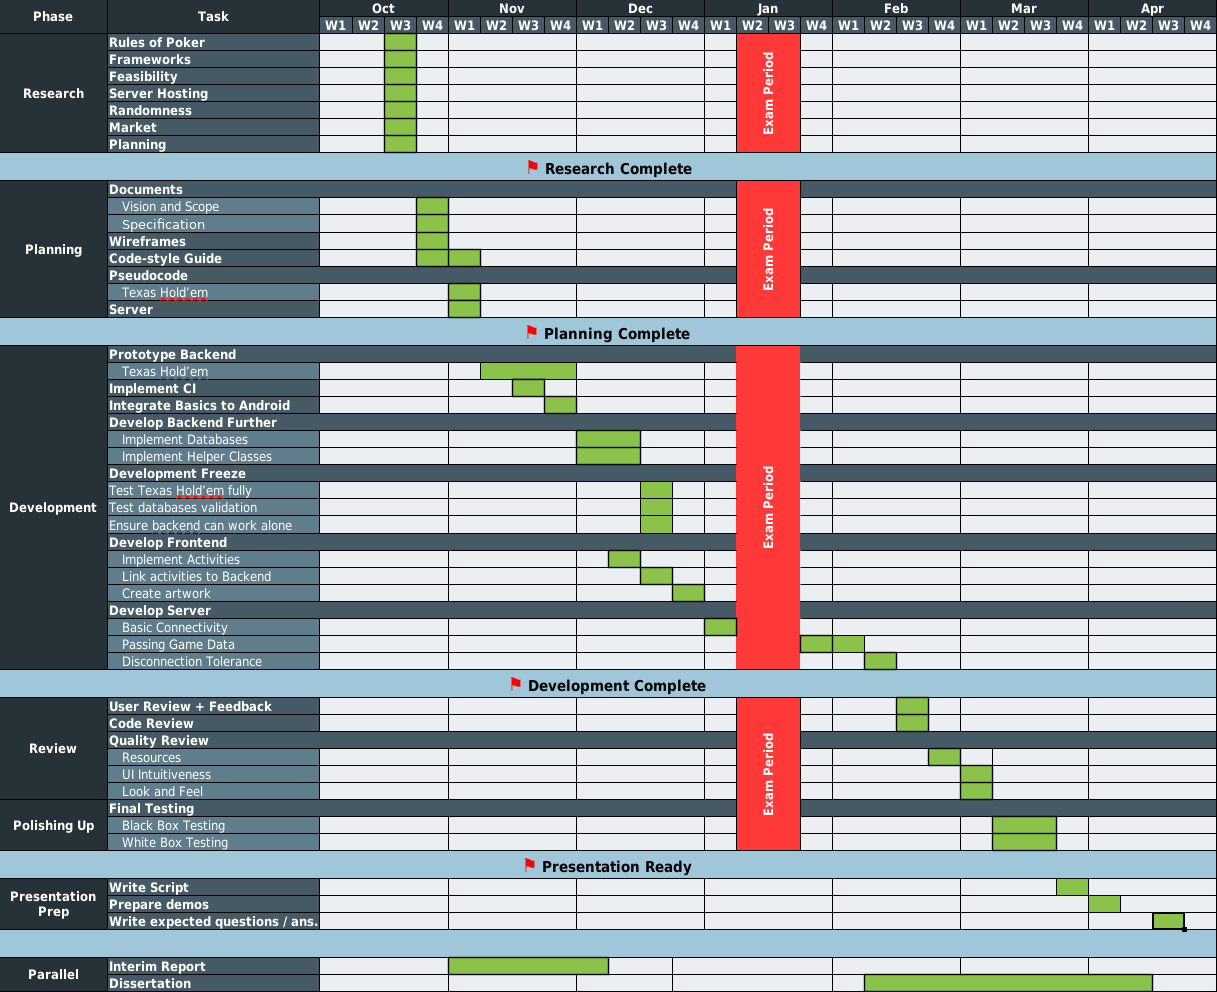
\includegraphics[width=1.22\textwidth]{gantt_chart.png}}
	\end{center}
\end{landscape}




\end{document}



